\documentclass{article}

\usepackage[colorlinks=true, urlcolor=blue]{hyperref}
\usepackage{minted}
\usepackage{multirow}
\usepackage{graphicx}
\usepackage{subcaption}
\usepackage[backend=bibtex]{biblatex}

\addbibresource{references.bib}

\begin{document}
	
\title{Analysis and Prediction of Multi-Dimensional data for Genetic Syndromes Using Machine Learning}
\author{Alexandre Silva}
\date{\today}
	
\maketitle

\section{Introduction}

As requested by the company, a pipeline was constructed to explore the embeddings data and extract insights from there. Many challenges were faced during the process, but we reached good results which are going to be presented here.
By means of easing the process of understanding the data and effectively creating the classification model, we employed the following tools: Jupyter Notebook (for a priori analysis), Python, Streamlit, Scikit-Learn, Imbalanced-Learn, Pandas and Numpy.
At the end of the project, we created a pipeline extracting all the knowledge we gained from our a priori analysis done in jupyter notebooks. With this pipeline, we connected the parts in an easy to use dashboard with Streamlit which is accessible via this link: \href{https://apollo-project.streamlit.app/}{https://apollo-project.streamlit.app/}. Also, the code and experiments can be seen in this github repository: \href{https://github.com/Dpbm/apollo-project}{https://github.com/Dpbm/apollo-project}; As well as in the zip file within the attachments.
In this document, we aim to show our thoughts, methodologies and insights we extracted during the process. In Section \ref{sec1}, we’re going to present how the data was parsed, transformed and analyzed, what we found at that step; In Section \ref{sec2}, we’re going to discuss the model creation, training and evaluation; In Section \ref{sec3}, we’re going to show the output metrics and analyze them in respect to the data; Finally, In Section \ref{sec4} we’re going to give overall insights and briefly discuss future works and improvements.

\section{Data Analysis} \label{sec1}

As the provided data was a pickle file, the first step was to open it and understand its internal structure. It was known that it was a python Dictionary with 3 levels of data following the structure as shown below in JSON \ref{structure} .

\label{structure}
\begin{minted}{js} 
	 { 'syndrome_id': {
		'subject_id': {
			'image_id': [
				320-dimensional embedding
			]
		}
	}}
\end{minted}

However, we did not know exactly how the ids looked liked nor the embedding. So first of all, we employed the pythons built-in methods for dictionaries \textit{.values()} and \textit{.keys()} for each JSON level, aiming to get a grasp of how the syndromes, subjects and images were distributed. To ease the visualization and allow us to find inconsistencies within the data, we extract the object characteristics to a \textit{Pandas DataFrame}, this way we could manipulate the data as we wanted efficiently. For that, we used the code Python. \ref{extract} in our Notebook.

\newpage

 
\label{extract}
\begin{minted}{python} 
	mapping = pd.DataFrame(columns=("syndrome", "subject", "image", 
	                          "image_size", "max_value", "min_value"))
	
	index = 0
	for syndrome in dataset.keys():
		subjects = dataset[syndrome].keys()
		print("-"*20)
		print(f"Looking for Syndrome: `{syndrome}`")
		print(f"Total subjects: {len(subjects)}")
	
		amount_of_images = set()
		for subject in subjects:
			images = dataset[syndrome][subject].keys()
			amount_of_images.add(len(images))
			total_images_per_subject = 0
	
			for image_id in images:
				image = dataset[syndrome][subject][image_id]
				mapping.loc[index] = {
						"syndrome":syndrome, 
						"subject":subject, 
						"image":image_id, 
						"image_size":len(image), 
						"max_value":max(image), 
						"min_value":min(image)
					}
				index += 1
				total_images_per_subject += 1
			print(f"""
				Number of images for {subject} subject: 
					{total_images_per_subject}""")
		print(f"Overall amount of images: {list(amount_of_images)}")
	print("#"*20)
	mapping.head()
\end{minted}

Using this DataFrame, we could easily filter for \textit{Nan} values, embeddings without the correct amount of dimensions ($320$), we could also understand how many images per syndrome or either per subject the dataset has. Another interesting characteristic we extracted was the min and max values for each embedding, we did it aiming to see if there were any data that could be too far away in some dimension or either too close, giving us the ability to plot the distribution later.

Now for the embeddings, we had to convert the dictionary data into a more suitable format, in this case we moved the embeddings array into a \textit{numpy ndarray}. This new structure allowed us to apply transformations, and plot it as we wished with ease. The final shape of this condensed block of embeddings was $(1116, 320)$, being in total $1116$ images/rows in total. During the proccess we also checked for invalid data, like \textit{np.nan} and \textit{np.inf}, getting hid of them using \textit{np.nan\_to\_num}. The algorithm looked like following (Python. \ref{ndarray}).


\label{ndarray}
\begin{minted}{python} 
	EACH_ARRAY_SIZE=320 # as described by the problem
	total_images = mapping.shape[0]
	
	print(f"Creating array of {(total_images,EACH_ARRAY_SIZE)}")
	data_arr = np.ndarray((total_images,EACH_ARRAY_SIZE),dtype=np.float32)
	
	for i,row in mapping.iterrows():
		syndrome,subject,image_i = row["syndrome"],row["subject"],row["image"]
		image = dataset[syndrome][subject][image_i]
		data_arr[i] = np.nan_to_num(image)
\end{minted}

This size of this condensed data was measured and it consumed $\approx 1Mb$.

Notice that we ensured that the generated array was matching the indexes in the DataFrame by iterating over rows and using the row index as the array index.

\subsection{DataFrame analysis}

Using \textit{Pandas} built-in methods, we started checking for incongruence. Running the \textit{.describe()} method, we were allowed to look for numerical incongruence within the data, but none was found as show at Table.\ref{table-df}.

\begin{table}[!h]
	\begin{center} 

		
		\begin{tabular}{ |c|c|c|c| } 
			\hline
			 & image size	& max value &	min value \\
			\hline
			count	& 1116.0  & 1116.000000	& 1116.000000 \\
			mean    & 320.0	  & 3.514369	& -3.549105 \\
			std	    & 0.0	  & 0.632139	& 0.643378 \\
			min	    & 320.0	  & 1.807156	& -7.986729 \\
			25\%	& 320.0	  & 3.064203	& -3.889321 \\
			50\%	& 320.0	  & 3.433821	& -3.481856 \\
			75\%	& 320.0	  & 3.898697	& -3.111340 \\
			max	    & 320.0	  & 7.798529	& -1.769748 \\
			\hline
		\end{tabular}
		\caption{Pandas \textit{.describe()} output for \textit{mapping DataFrame}.}
		\label{table-df}
	
	\end{center}
\end{table}

Image size had all instances with exactly $320$ dimensions, giving $std = 0.0$. Something similar happened for min and max value, the overall deviation was not alarming and in general the data has a solid proportion of values. It's likely that outliers may appear, but nothing that could implicate in future issues.

We also collected some primary information about the amount of syndromes, subjects and images shown in Python.\ref{overall}.

\newpage

\label{overall}
\begin{minted}{python} 
	print("-=-Over all statistics-=-")
	print(f"Number of syndromes: {len(mapping.syndrome.unique())}")
	print(f"Number of subjects: {len(mapping.subject.unique())}")
	print(f"Number of images: {len(mapping)}")
	
	"""
	Output
	---------------
	
	
	-=-Over all statistics-=-
	Number of syndromes: 10
	Number of subjects: 941
	Number of images: 1116
	
	"""
\end{minted}

At this point, we started implementing the dashboard using \textit{Streamlit} and also extracted a few more statistics from it Python.\ref{statistics}.

\label{statistics}
\begin{minted}{python} 
def get_overall_statistics(df:pd.DataFrame) -> Statistics:
	"""Get Statistics from dataframe.""" 
	
	total_images = df.shape[0]
	syndromes = df.syndrome.unique()
	total_syndromes = len(syndromes)
	total_subjects = len(df.subject.unique())
	
	min_max_value = df.max_value.min()
	max_max_value = df.max_value.max()
	avg_max_value = df.max_value.mean()
	median_max_value = df.max_value.median()
	
	min_min_value = df.min_value.min()
	max_min_value = df.min_value.max()
	avg_min_value = df.min_value.mean()
	median_min_value = df.min_value.median()
	
	statistics = {
		"total_images":total_images,
		"total_syndromes":total_syndromes,
		"total_subjects":total_subjects,
		"min_max_value":min_max_value,
		"max_max_value":max_max_value,
		"avg_max_value":avg_max_value,
		"median_max_value":median_max_value,
		"min_min_value":min_min_value,
		"max_min_value":max_min_value,
		"avg_min_value":avg_min_value,
		"median_min_value":median_min_value,
		"syndromes_amount_of_subjects":{},
		"syndromes_amount_of_images":{},
	}
	
	
	for syndrome in syndromes:
		amount_of_subjects = len(df[df.syndrome == syndrome].subject.unique())
		statistics["syndromes_amount_of_subjects"][syndrome] = amount_of_subjects
	
	for syndrome in syndromes:
		amount_of_images = len(df[df.syndrome == syndrome].image)
		statistics["syndromes_amount_of_images"][syndrome] = amount_of_images
	
	return statistics
\end{minted}

And with this new object we visualized it on the dashboard as on Figure.\ref{statistics-dashboard}.

\newpage
\begin{figure}[H] 
	\centering
	\begin{subfigure}{0.8\textwidth}
		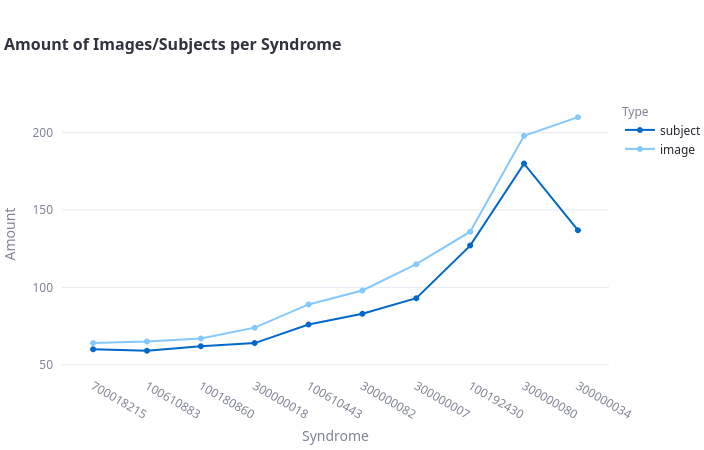
\includegraphics[width=\linewidth]{assets/images-subjects-per-syndrome}
		\caption{Plot showing the amount of images and subjects per syndrome.}
		\label{subjects-images}
	\end{subfigure}
	\vfill 
	\begin{subfigure}{0.8\textwidth}
		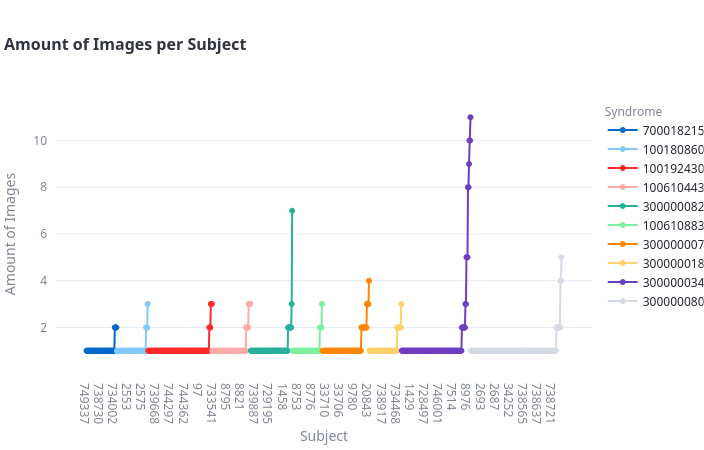
\includegraphics[width=\linewidth]{assets/images-per-subject}
		\caption{Shows the amount of images per subject.}
		\label{imgs-per-subject}
	\end{subfigure}
	\vfill
	\begin{subfigure}{0.8\textwidth}
		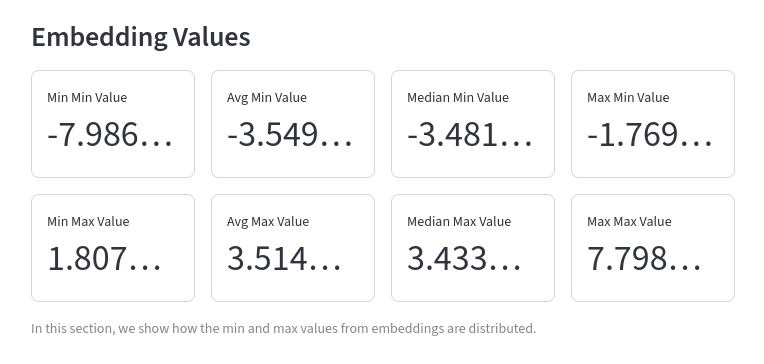
\includegraphics[width=\linewidth]{assets/embeddings-distribution}
		\caption{The distribution between embedding min and max values.}
	\end{subfigure}
	
	\caption{New Statistics shown on the \textit{Streamlit} dashboard.}
	\label{statistics-dashboard}
\end{figure}

The plots on Figure.\ref{statistics-dashboard} shown us that the input data was imbalanced across different labels. While some had $\approx 200$ images, others had $\approx 50$, being an alarming factor. To overcome this, we focused on \textit{under-sampling} techniques. For this case, we tested different approaches, but the one who best fit our needs was \textit{RepeatedEditedNearestNeighbours}, method available in the \textit{Imbalanced-Learn} Python package. This method uses the \textit{KNN(k-nearest neighbors)} algorithm to clean the noisy data, prevailing the clusters and creating spaces between them. A better approach would be \textit{data augmentation}, but we don't know exactly how does the data looked like previously, so it was not suitable for our case. 

An also interesting to notice fact present on the plot Figure.\ref{subjects-images}, which is also affirmed by Figure.\ref{imgs-per-subject}, is the pair subject-image. The plot behavior follows the expected rule that, with more people having a syndrome (subject), more images we'll have. So, those syndrome with less images might be considered rare. Due to this fact, it may be the reason for the imbalanced dataset, being sometimes difficult to find data on the wild.

\subsection{T-SNE}

Since we had a $320$-dimensional embedding, it is not possible to plot it right away, so we needed a different approach. The \textit{T-SNE} is an algorithm designed to reduce the dimensionality of data, as done by the well-known algorithm \textit{PCA}, but preserving its local structure.

We applied this algorithm through our experiments, as a way to visualize the clusters. We also applied it to test the under-sampling techniques as shown at Figure.\ref{tsne-plots}.

\newpage
\begin{figure}[H] 
	\centering
	\begin{subfigure}{0.45\textwidth}
		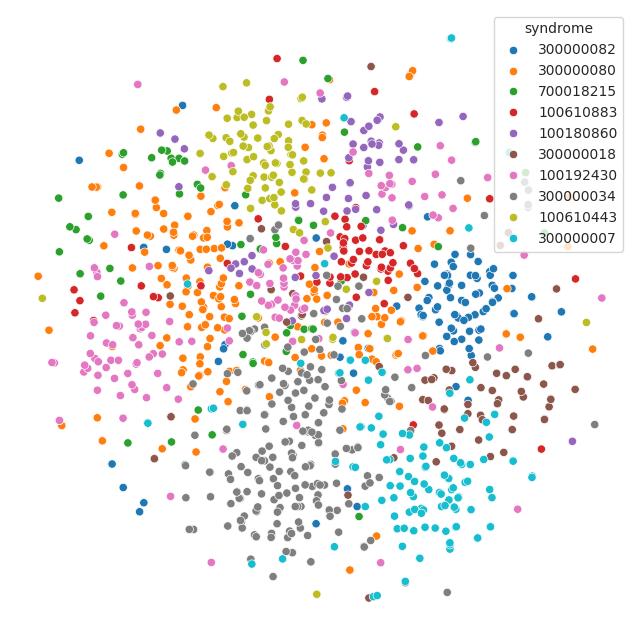
\includegraphics[width=\linewidth]{assets/tsne-raw}
		\caption{Plot showing the noisy data using parameters: $learning-rate=800; perplexity=50; init=pca$.}
		\label{dirty-data}
	\end{subfigure}
	\hfill
	\begin{subfigure}{0.45\textwidth}
		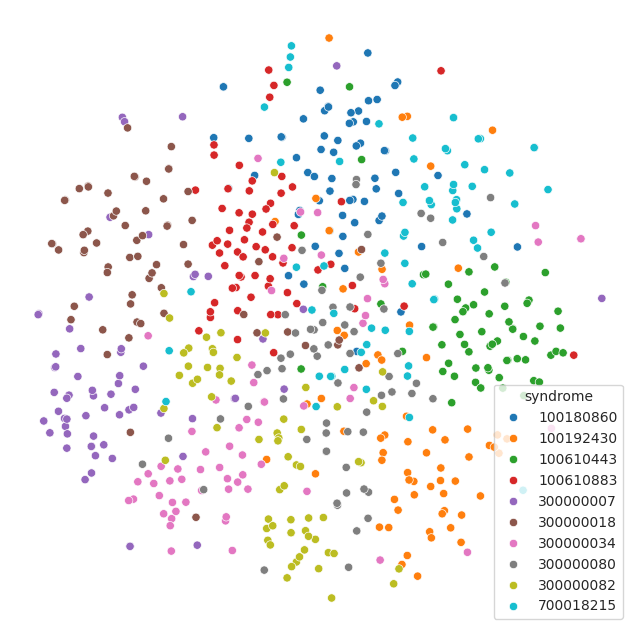
\includegraphics[width=\linewidth]{assets/tsne-random}
		\caption{Plot for under-sampling using Random Sampling.}
		\label{undersampling-random}
	\end{subfigure}
	\vfill
	\begin{subfigure}{0.45\textwidth}
		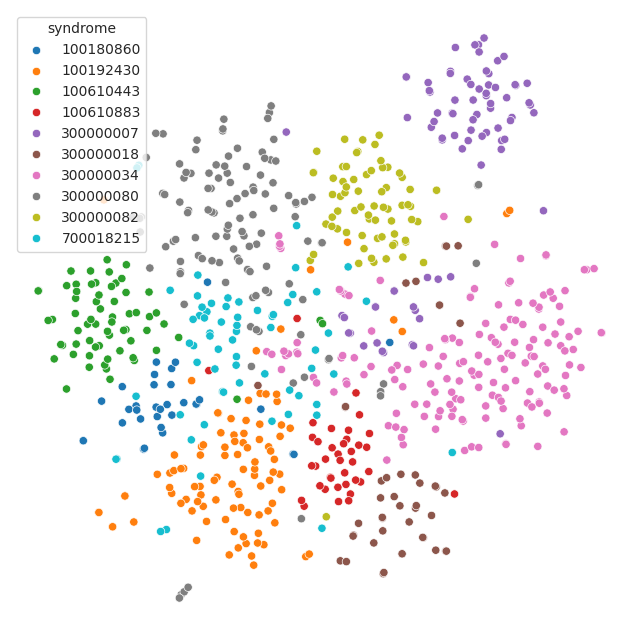
\includegraphics[width=\linewidth]{assets/tsne-allknn}
		\caption{Plot using under-sampling AllKNN method.}
		\label{undersampling-allknn}
	\end{subfigure}
	\hfill
	\begin{subfigure}{0.45\textwidth}
		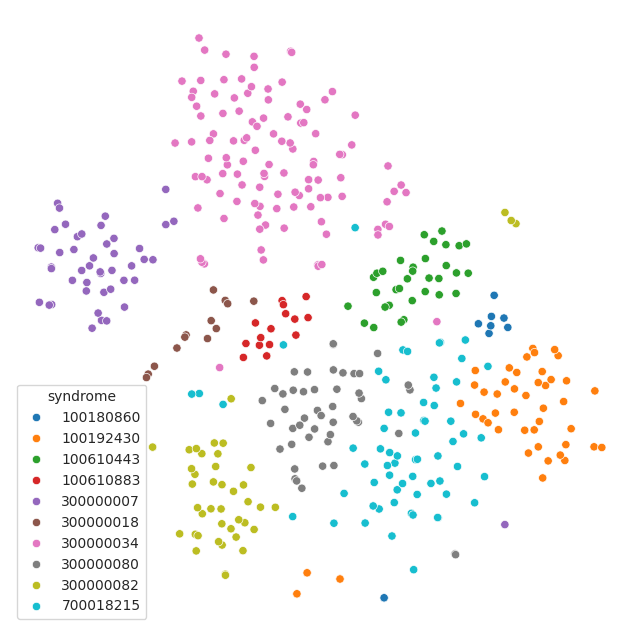
\includegraphics[width=\linewidth]{assets/tsne-edited}
		\caption{Plot using under-sampling RepeatedEditedNearestNeighbours method.}
		\label{undersampling-editedknn}
	\end{subfigure}
	
	\caption{T-SNE plots for different techniques.}
	\label{tsne-plots}
\end{figure}

At Figure.\ref{dirty-data} we tweaked the T-SNE for the dirty input data, however it is usually complicated to get good representations this way, even though some clusters may appear. On the other hand, using the under-sampling techniques, we were able to clean the data and get better visualization as shown in Figures.[\ref{undersampling-random}, \ref{undersampling-allknn}, \ref{undersampling-editedknn}]. The last two were the bests, but the \textit{RepeatedEditedNearestNeighbours} was shown as the best choice,cleaning the data at granular level.

Before each run, the data is normalized using $l2$ normalization, to ensure that the values are within the bounds $[-1,1]$ as required by \textit{T-SNE}.

\section{Model Setup} \label{sec2}

For the model, we used KNN (k-nearest neighbors) algorithm, being one of the most common algorithms for classifying points by their proximity.

In this experiment, we tested two different metrics for KNN, being them \textit{cosine} and \textit{euclidean}, also different parameters of \textit{n-neighbors}, ranging from $1$ to $15$. For this task, we used \textit{GridSearchCV} from \textit{Scikit-Learn}, to test these parameters and give a rank with the best based on accuracy and split across $10$ folds for Cross-Validation.

The outcomes pointed $k=1$ for \textit{cosine} and $k=6$ for \textit{euclidean}, which are low than expected but it is due to the dataset reduction after under-sampling.

With that, the model was trained using the optimal parameters for both \textit{cosine} and \textit{euclidean}, so in total we had $2$ models being trained.

The data used was the resampled dataset we created in Section.\ref{sec1} split into train and test being $80-20\%$ respectively. Then, the training batch was separated into $k=10$ folds for Cross-Validation and the remaining test portion was used later for evaluation.

To keep the data evenly spread across folds and splits, we used \textit{StratifiedKFold} and set the parameter \textit{stratify} for \textit{train\_test\_split}.

\section{Performance Metrics} \label{sec3}

To ensure our model was doing generalizing correctly the instances and evolving, we used different metrics and calculated that for each fold and after evaluation. The used metrics here are: accuracy, recall (micro), precision (micro), f1 (per label), ROC-AUC (OVR) and Top-K. In addition, we calculated a confusion matrix for each fold and evaluation.

For ROC-AUC per fold, we calculated and averaged that at the end, so we got, indeed, the average ROC-AUC per label across all $k$ folds. The method used for that is discussed in \cite{_receiver} and \cite{shen_2017_how}.

After Doing that, the results are shown in Figure.[\ref{results-per-fold}, \ref{results-overall}] and Table.\ref{table-eval}.

\newpage
\begin{figure}[H] 
	\centering
	\begin{subfigure}{0.45\textwidth}
		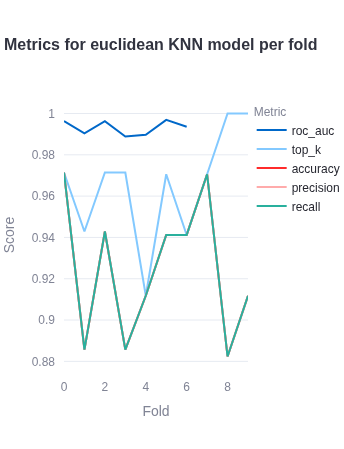
\includegraphics[width=\linewidth]{assets/euclidean-per-fold}
		\caption{Metrics for Euclidean model per fold.}
		\label{euclidean-per-fold}
	\end{subfigure}
	\hfill
	\begin{subfigure}{0.45\textwidth}
		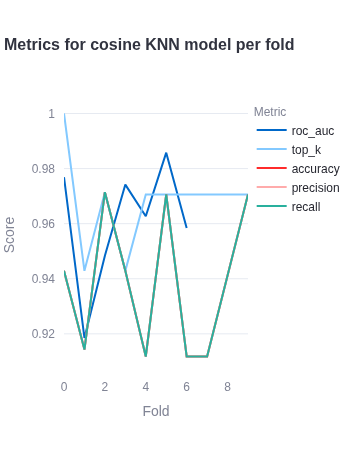
\includegraphics[width=\linewidth]{assets/cosine-per-fold}
		\caption{Metrics for cosine model per fold.}
		\label{cosine-per-fold}
	\end{subfigure}
	\vfill
	\begin{subfigure}{0.45\textwidth}
		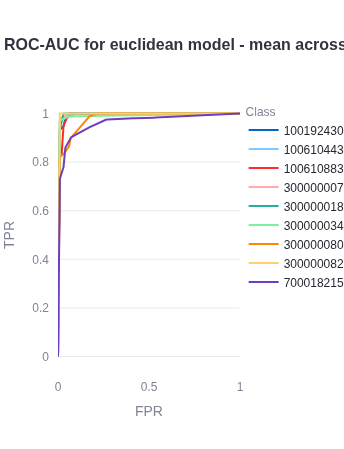
\includegraphics[width=\linewidth]{assets/roc-euclidean-per-fold}
		\caption{Mean ROC-AUC across folds for Euclidean model per syndrome.}
		\label{roc-per-fold-euclidean}
	\end{subfigure}
	\hfill
	\begin{subfigure}{0.45\textwidth}
		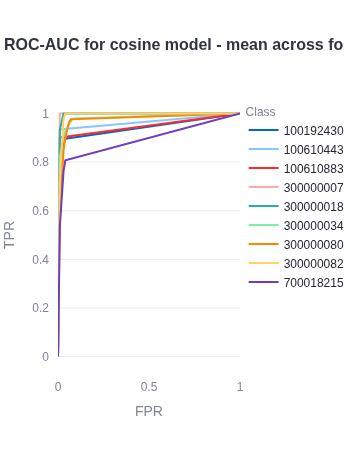
\includegraphics[width=\linewidth]{assets/roc-cosine-per-fold}
		\caption{Mean ROC-AUC across folds for cosine model per syndrome.}
		\label{roc-per-fold-cosine}
	\end{subfigure}
	
	\caption{Output metrics per fold.}
	\label{results-per-fold}
\end{figure}

\newpage
\begin{figure}[H] 
	\centering
	\begin{subfigure}{0.45\textwidth}
		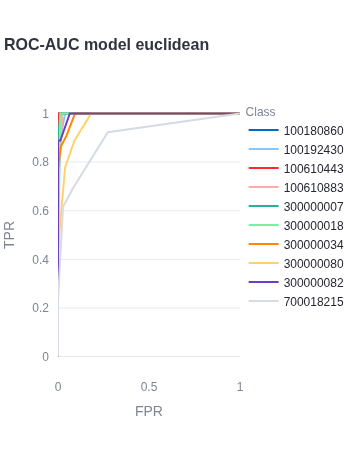
\includegraphics[width=\linewidth]{assets/roc-overall-euclidean}
		\caption{ROC-AUC for Euclidean model after evaluation.}
		\label{roc-euclidean}
	\end{subfigure}
	\hfill
	\begin{subfigure}{0.45\textwidth}
		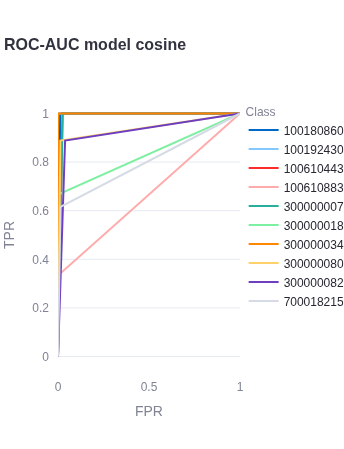
\includegraphics[width=\linewidth]{assets/roc-overall-cosine}
		\caption{ROC-AUC for cosine model after evaluation.}
		\label{roc-cosine}
	\end{subfigure}
	\caption{ROC-AUC for model after evaluation.}
	\label{results-overall}
\end{figure}

\begin{table}[!h]
	\begin{center} 
		
		
		\begin{tabular}{ |c|c|c| } 
			\hline
			& Euclidean & Cosine \\
			\hline
			roc\_auc & 0.9847 & 0.9132 \\
			top\_k & 0.9186 & 0.9186 \\
			accuracy & 0.8140 & 0.8837 \\
			precision & 0.8140 & 0.8837 \\
			recall & 0.8140 & 0.8837 \\
			\hline
		\end{tabular}
		\caption{Evaluation metrics for each model.}
		\label{table-eval}
		
	\end{center}
\end{table}

The results are pretty decent given the amount of images used for training. The model reached a really good precision and it's ROC-AUC curve is high.

Comparing both models, Euclidean was the best, might be due to our transformed data that had a better proximity and a straight line was the best to find neighbors than comparing angles for cosine KNN metric.

One point that was observed, is that the AUC was lower for sparsed classes and classes with lower density, which is understandable since the model had less chance to understand these components as clusters. Finally, is also notable that the final performance kept faithful to what was seen during training, being always $\geq{0.8}$ for every metric.

\section{Conclusions} \label{sec4}

Data science projects are far from easy to implement, being required creativity, technique and knowledge to develop the best pipeline as possible.
For this very project, we could get some insights with relative simple graphs and data manipulation, however since the data was limited and not much context was given, the problem became more complex to tackle. For a better outcome for machine learning projects, much is required, but knowledge about the problem is one of the chief points to succeed.

During the development, we found that the data itself was imbalanced, requiring some sort of manipulating for under-sampling. After our analysis, it stacks out that it is likely that this occurred because the lack of some diseases data, especially those that are rare. Even though they are real and occur, the model may get confused and result in worse performance. The best option would be generating synthetic data some way, so it depends deeply on how the original data was alike.

For future works we would like to point some ideas to work with. First, using a different model for comparison like \textit{SVM} or even creating a \textit{Deep Neural Network}. Also, the \textit{T-SNE} is sometimes hard to understand, since it doesn't preserve the global relationship only local, so using \textit{UMAP} may be a better option and a got starting point for next experiments.


\printbibliography

\end{document}